\newpage
\chapter{DISEÑO DEL SISTEMA DE INFORMACIÓN}
	\vspace{2cm}	
	\begin{center}
	{\Large \textbf{FASE DE DESARROLLO} \par}
	\end{center}
	\vspace{5cm}
	
	\begin{center}
	\Huge \textbf{DSI}\par
	\end{center}


%\newpage
%
%\section{DSI 3: DISEÑO DE CASOS DE USO REALES}
%
%\subsection{Caso de Uso 1.1} 
%
%\subsubsection{Diagramas de Interacción (Comunicación y Secuencia)} 
%
%\subsubsection{Diagramas de Estados de las Clases} 
% 
%\subsubsection{Diagramas de Actividades} 
%
%
%\subsection{Caso de Uso 1.2}


\newpage
\section{DSI 4: DISEÑO DE CLASES}
\subsection{Diagrama de Clases}
\subsubsection{Museo}
\begin{figure}[H]
\centering
\centerline{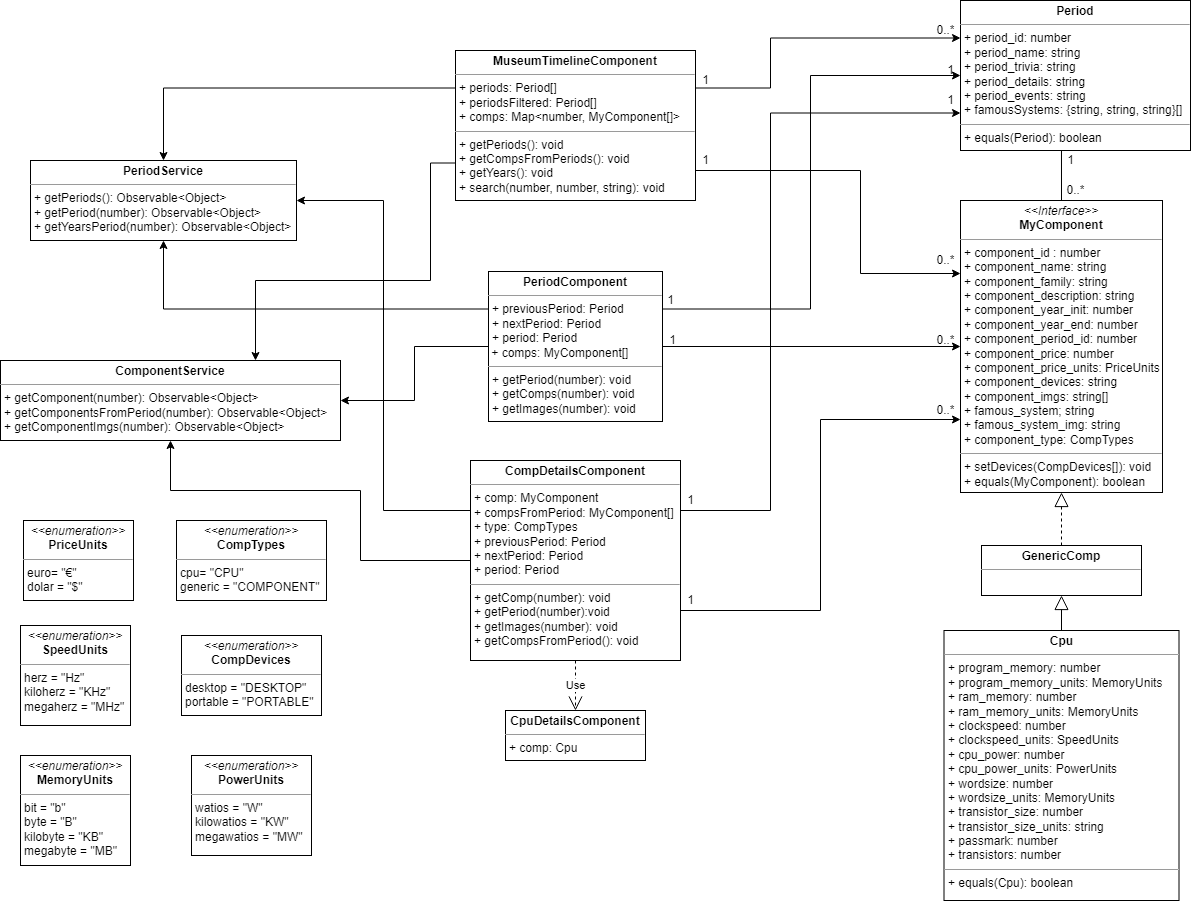
\includegraphics[scale=0.4]{dis-clases-museo}}
\caption{Diseño de clases: diagrama de clases del museo}
\end{figure}
\subsubsection{Administración del museo}
\begin{figure}[H]
\centering
\centerline{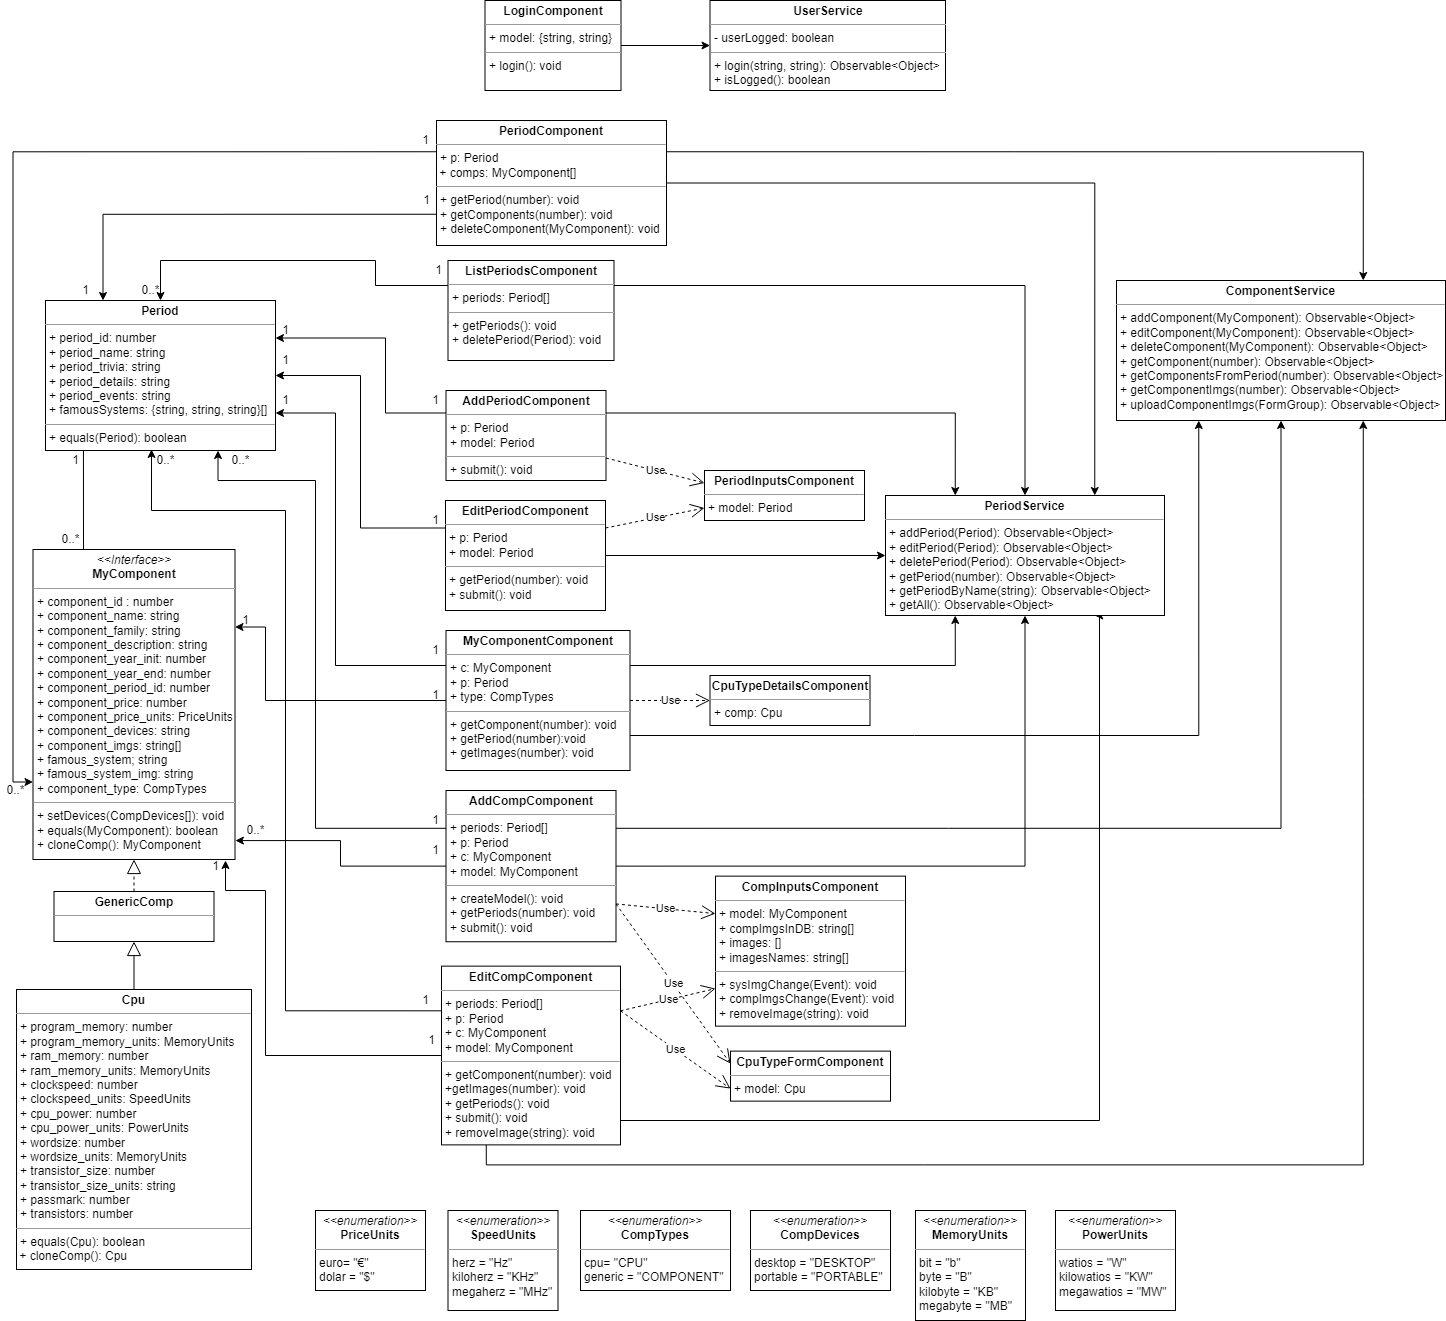
\includegraphics[scale=0.4]{dis-clases-admin}}
\caption{Diseño de clases: diagrama de clases de la administración del museo}
\end{figure}

\newpage
\section{DSI 5: DISEÑO DE LA ARQUITECTURA DE MÓDULOS DEL SISTEMA}

\subsection{Diagrama de paquetes}
\begin{figure}[H]
\centering
\centerline{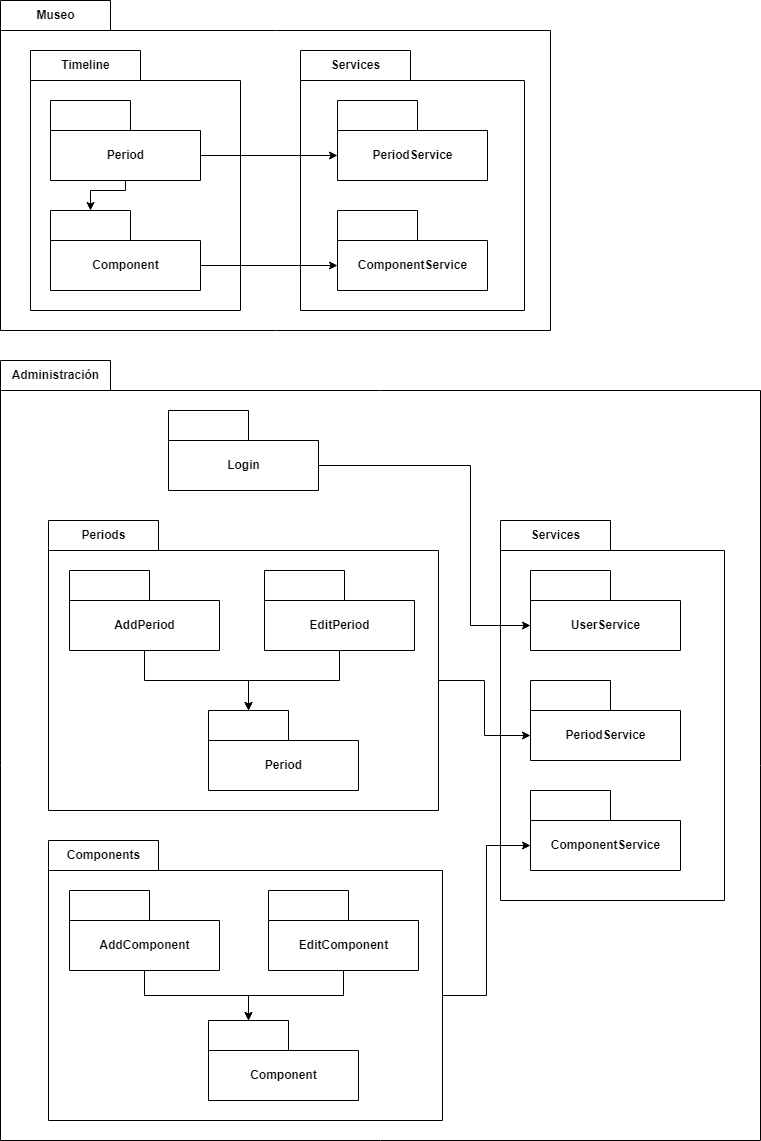
\includegraphics[scale=0.45]{paquetes}}
\caption{Diagrama de paquetes del sistema}
\end{figure}

%\subsection{Diagrama de componentes}

\subsection{Diagrama de despliegue}
\begin{figure}[H]
\centering
\centerline{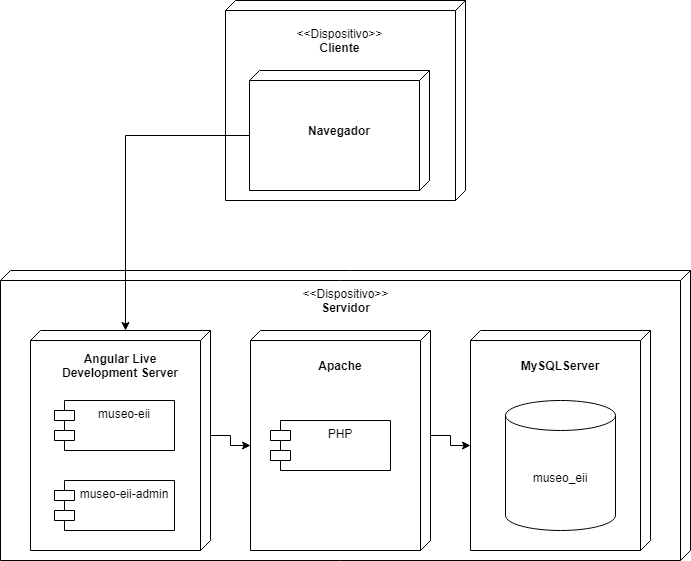
\includegraphics[scale=0.6]{despliegue}}
\caption{Diagrama de despliegue del sistema}
\end{figure}


\newpage
\section{DSI 6: DISEÑO FÍSICO DE DATOS}

\subsection{Descripción del SGBD Usado} 
Se ha creado una base de datos relacional, utilizando MySQL 8 como sistema gestor de bases de datos, debido a su gran popularidad en todo el mundo y en el desarrollo de aplicaciones con Angular y PHP.
\par La base de datos creada es museo-eii, y se compone de cinco tablas: 
\begin{itemize}
	\item periods: alamcena toda la información relativa a un periodo.
	\item components: contiene los datos que serían comunes a cualquier tipo de componente idependientemente de su tipo, como nombre, año de salida, precio, ect.
	\item components\_images: asigna el conjunto de imágenes de cada componente.
	\item cpus: almacena los datos específicos de una CPU, como la memoria RAM, la velocidad de reloj o el tamaño de palabra. El identificador de esta tabla referencia al elemento correspondiente de la tabla components, simulando así una herencia en la base de datos. Esta herencia simulada hace que la base de datos sea fácilmente ampliable si se añade un tipo de componente que no sea una CPU, ya que bastaría con añadir una nueva tabla con los campos necesarios que también referencie a components.
	\item administrator: almacena los datos de inicio de sesión del administrador (email y contraseña cifrada). En caso de que hubiera más usuarios que tuviesen que iniciar sesión se habría creado una base de datos exclusiva para almacenarlos, pero como en este caso solo existe un administrador, he decidido incluir esta tabla en la base de datos existente para este proyecto.
\end{itemize}
\subsection{Integración del SGBD en Nuestro Sistema} 
Para integrar el sistema con la base de datos se han creado tres servicios en angular: uno para periodos, otro para componentes y el último para el usuario. Estos tres servicios utilizan la librería HttpClient de Angular, que permite realizar peticiones HTTP para obtener o enviar datos al lado del servidor, donde se encuentran los archivos PHP que contienen las consultas que han de realizarse sobre la base de datos.
\subsection{Diagrama E--R} 
A continuación se muestra el diagrama entidad-relación de la base de datos del sistema, museo-eii:
\begin{figure}[H]
\centering
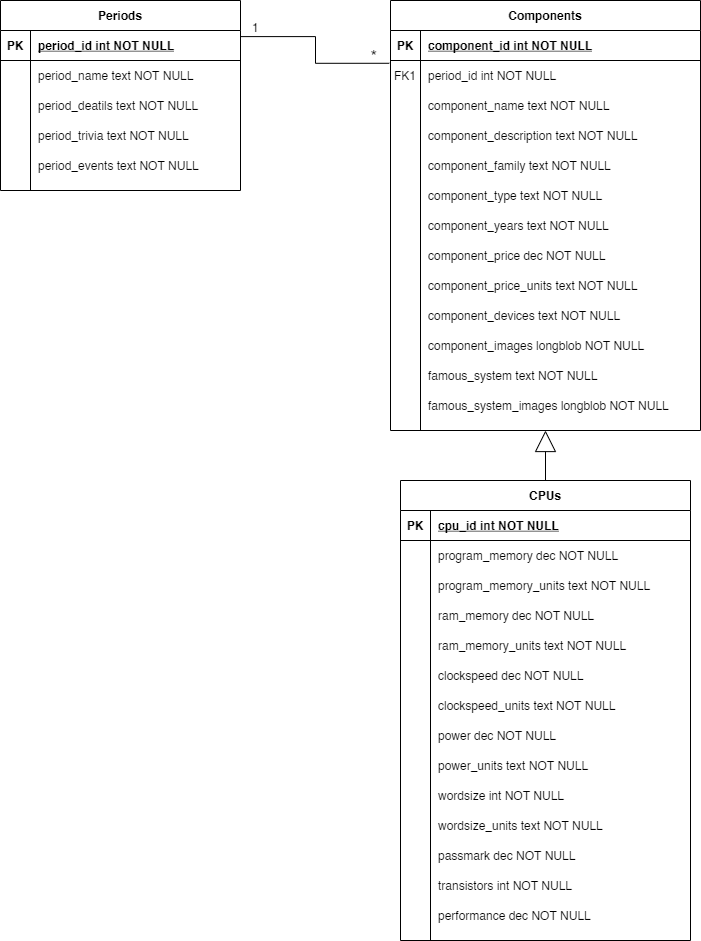
\includegraphics[scale=0.6]{diagrama_e-r}
\caption{Diagrama Entidad-Relación de la base de datos creada}
\end{figure}


%\newpage
%
%\section{DISEÑO DE LA INTERFAZ DE USUARIO}
%A continuación, se muestran las interfaces definitivas de la aplicación web.
%\subsubsection{Museo}
%\begin{figure}[H]
%\centering
%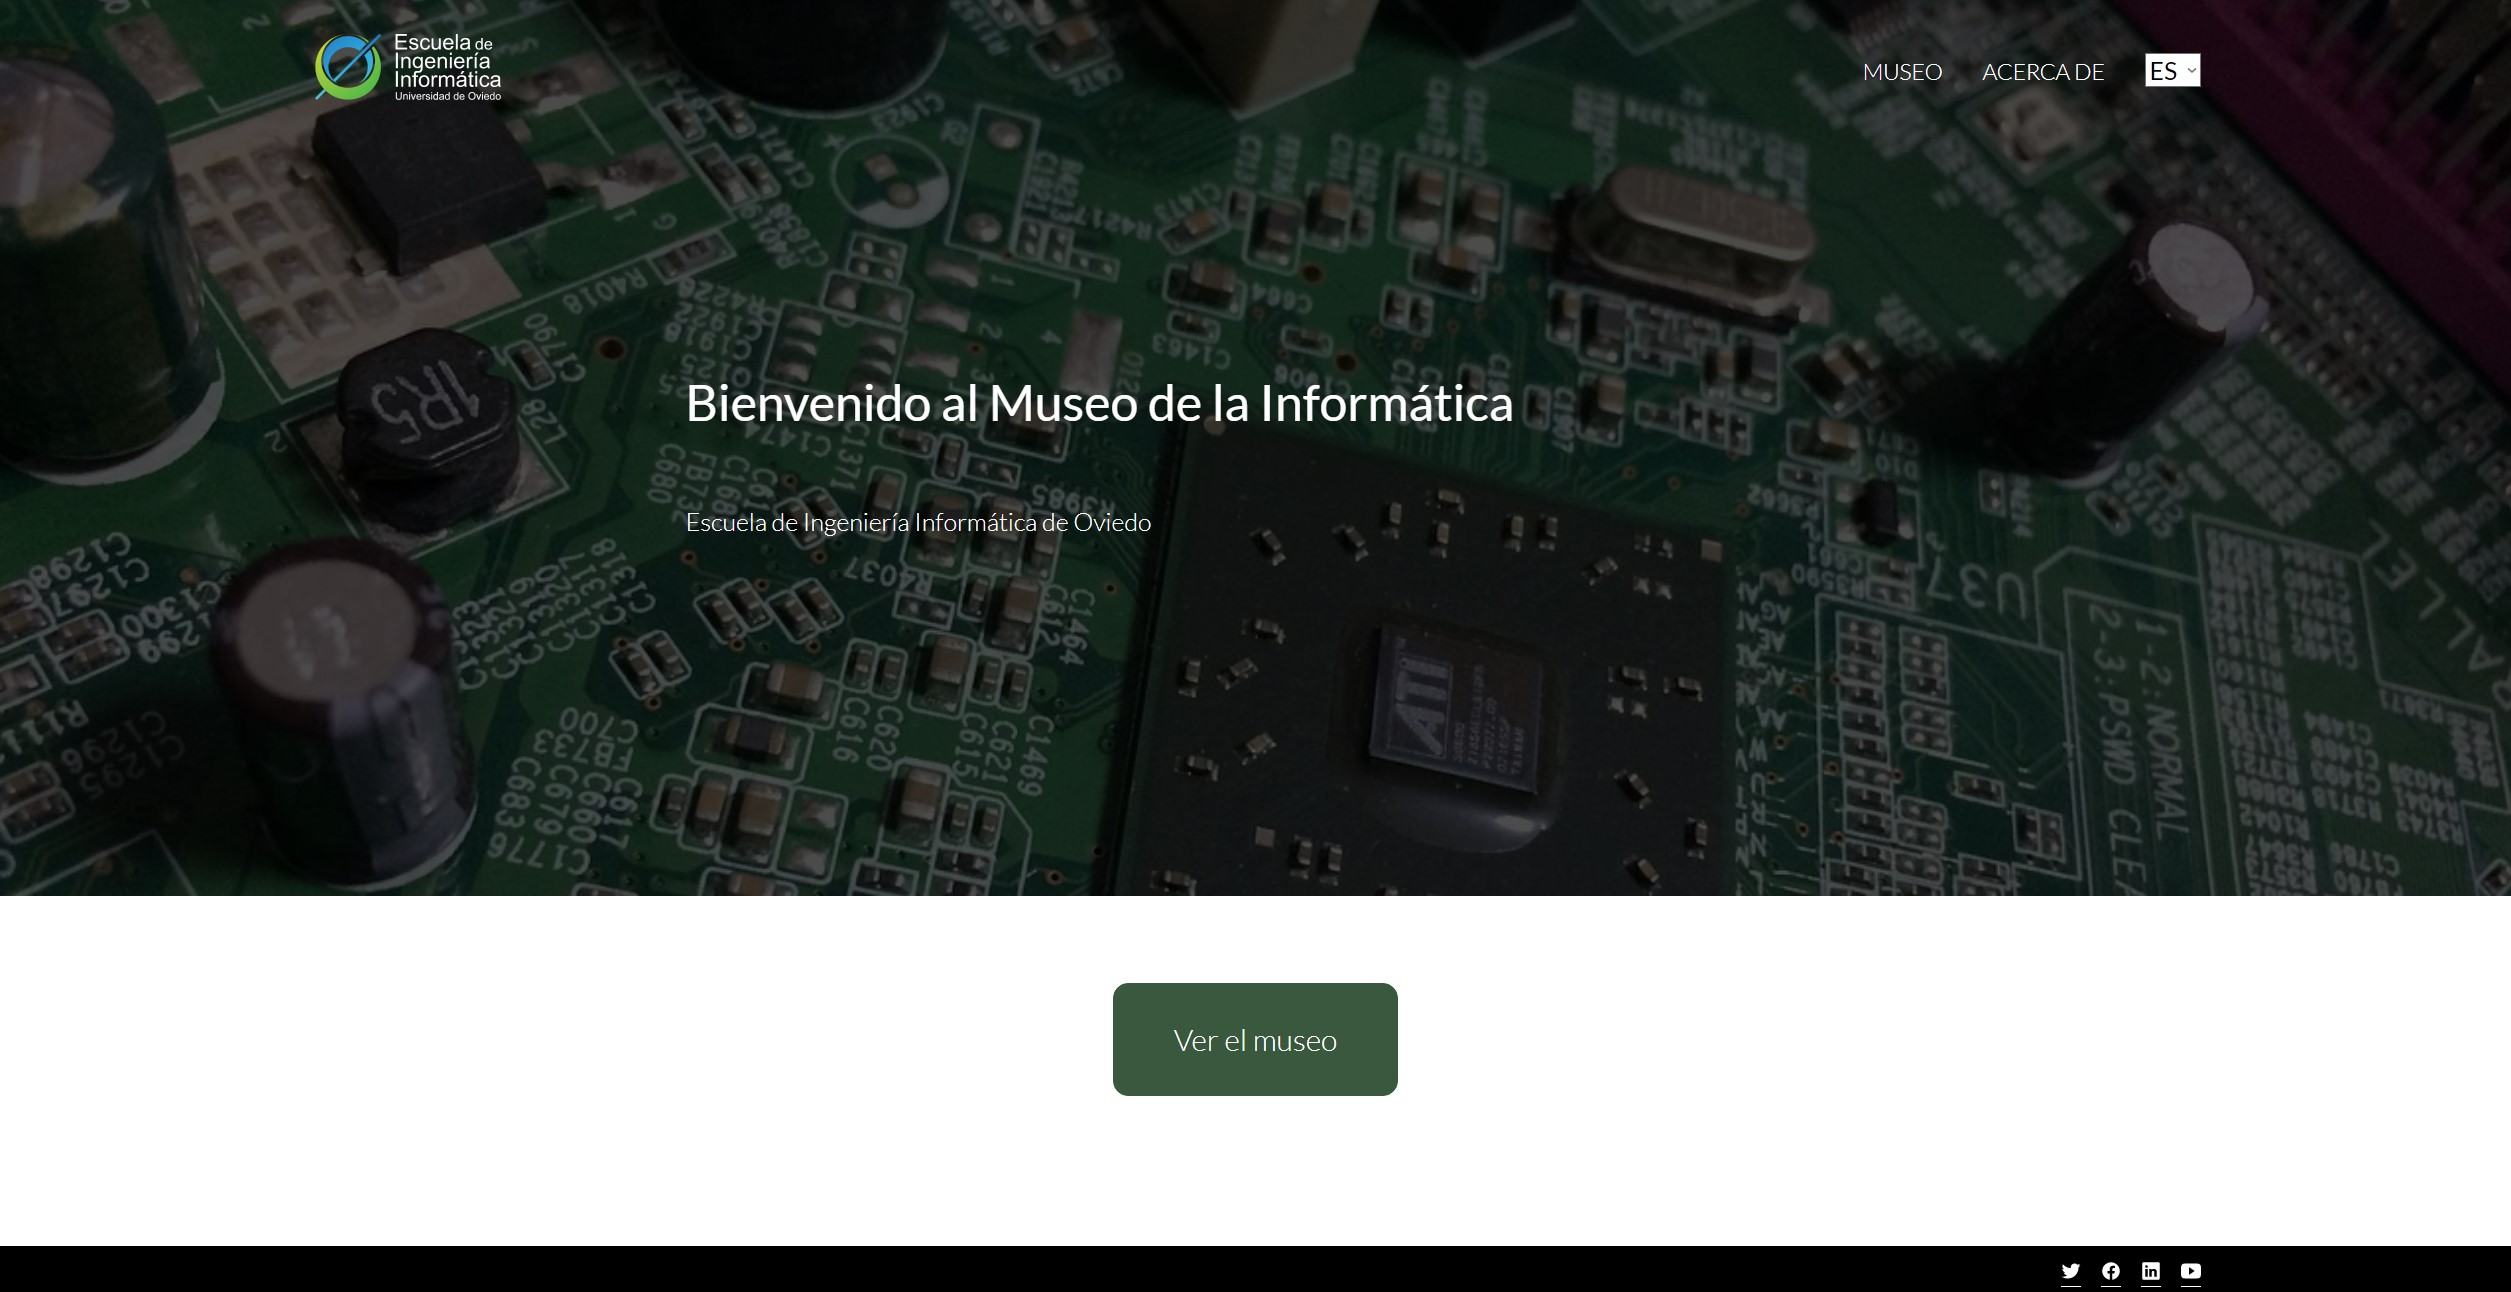
\includegraphics[scale=0.25]{homeIUDef}
%\caption{Página de inicio}
%\end{figure}
%\begin{figure}[H]
%\centering
%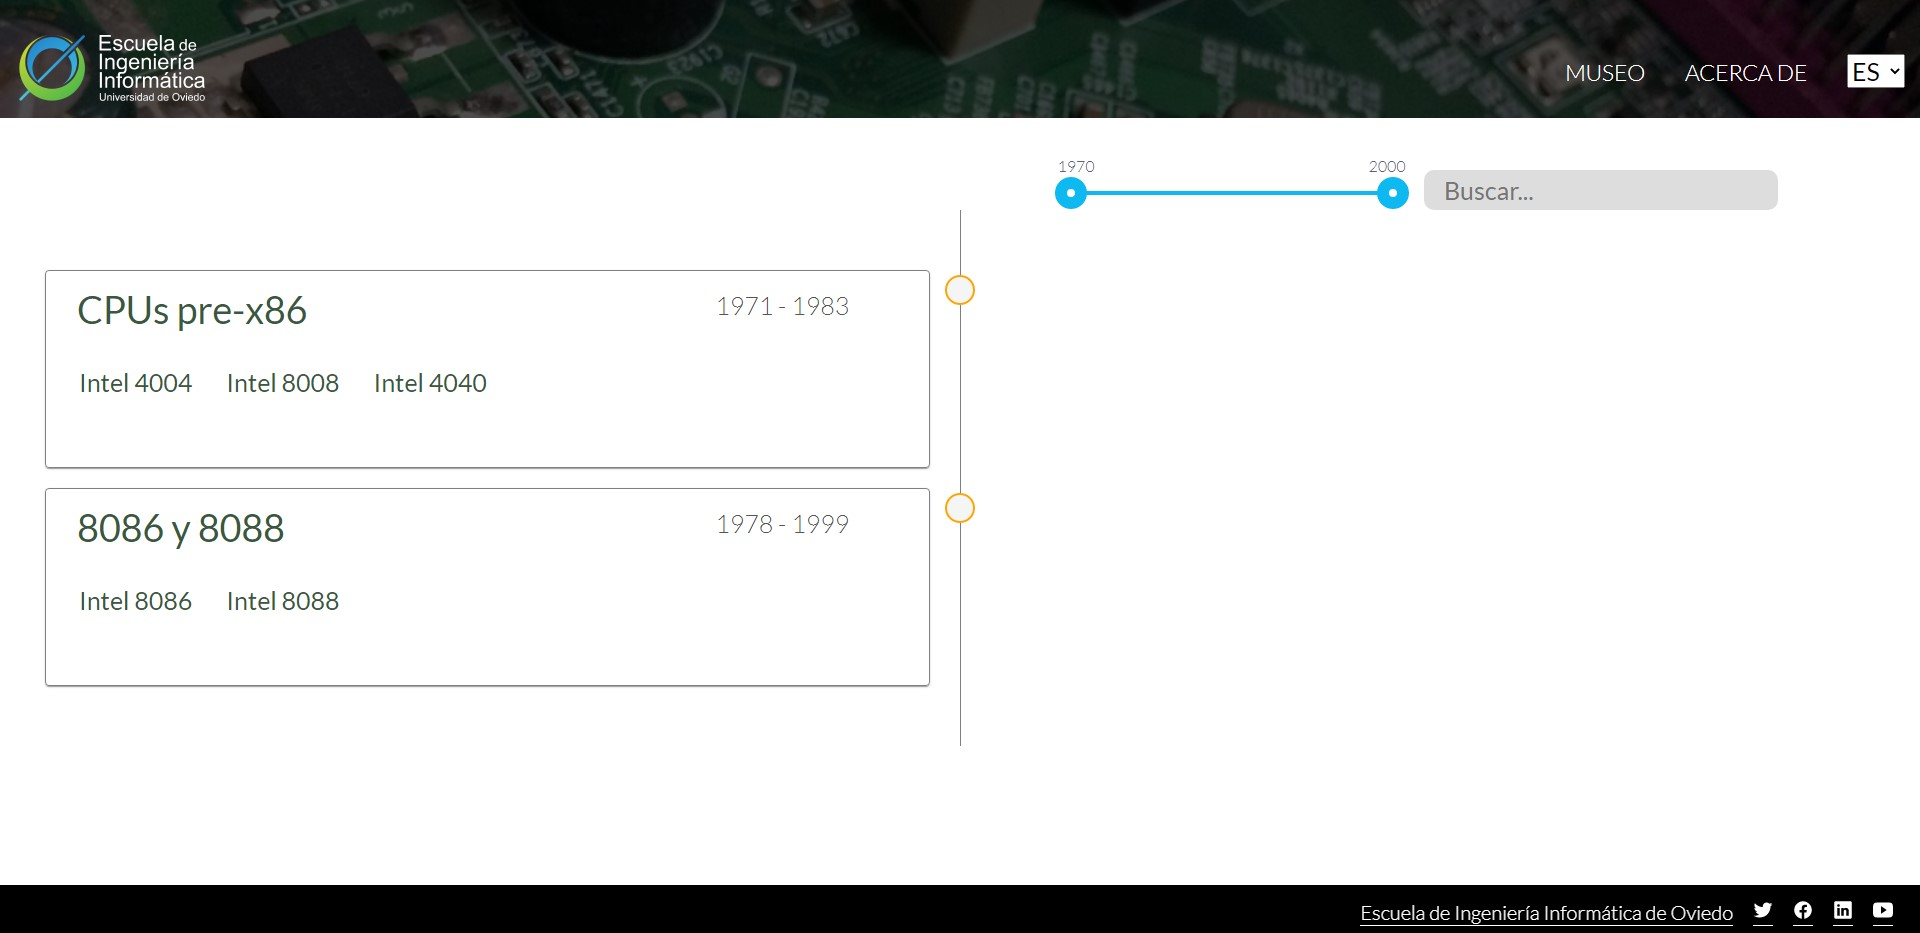
\includegraphics[scale=0.25]{museoIUDef}
%\caption{Página de la vista general del museo}
%\end{figure}
%\begin{figure}[H]
%\centering
%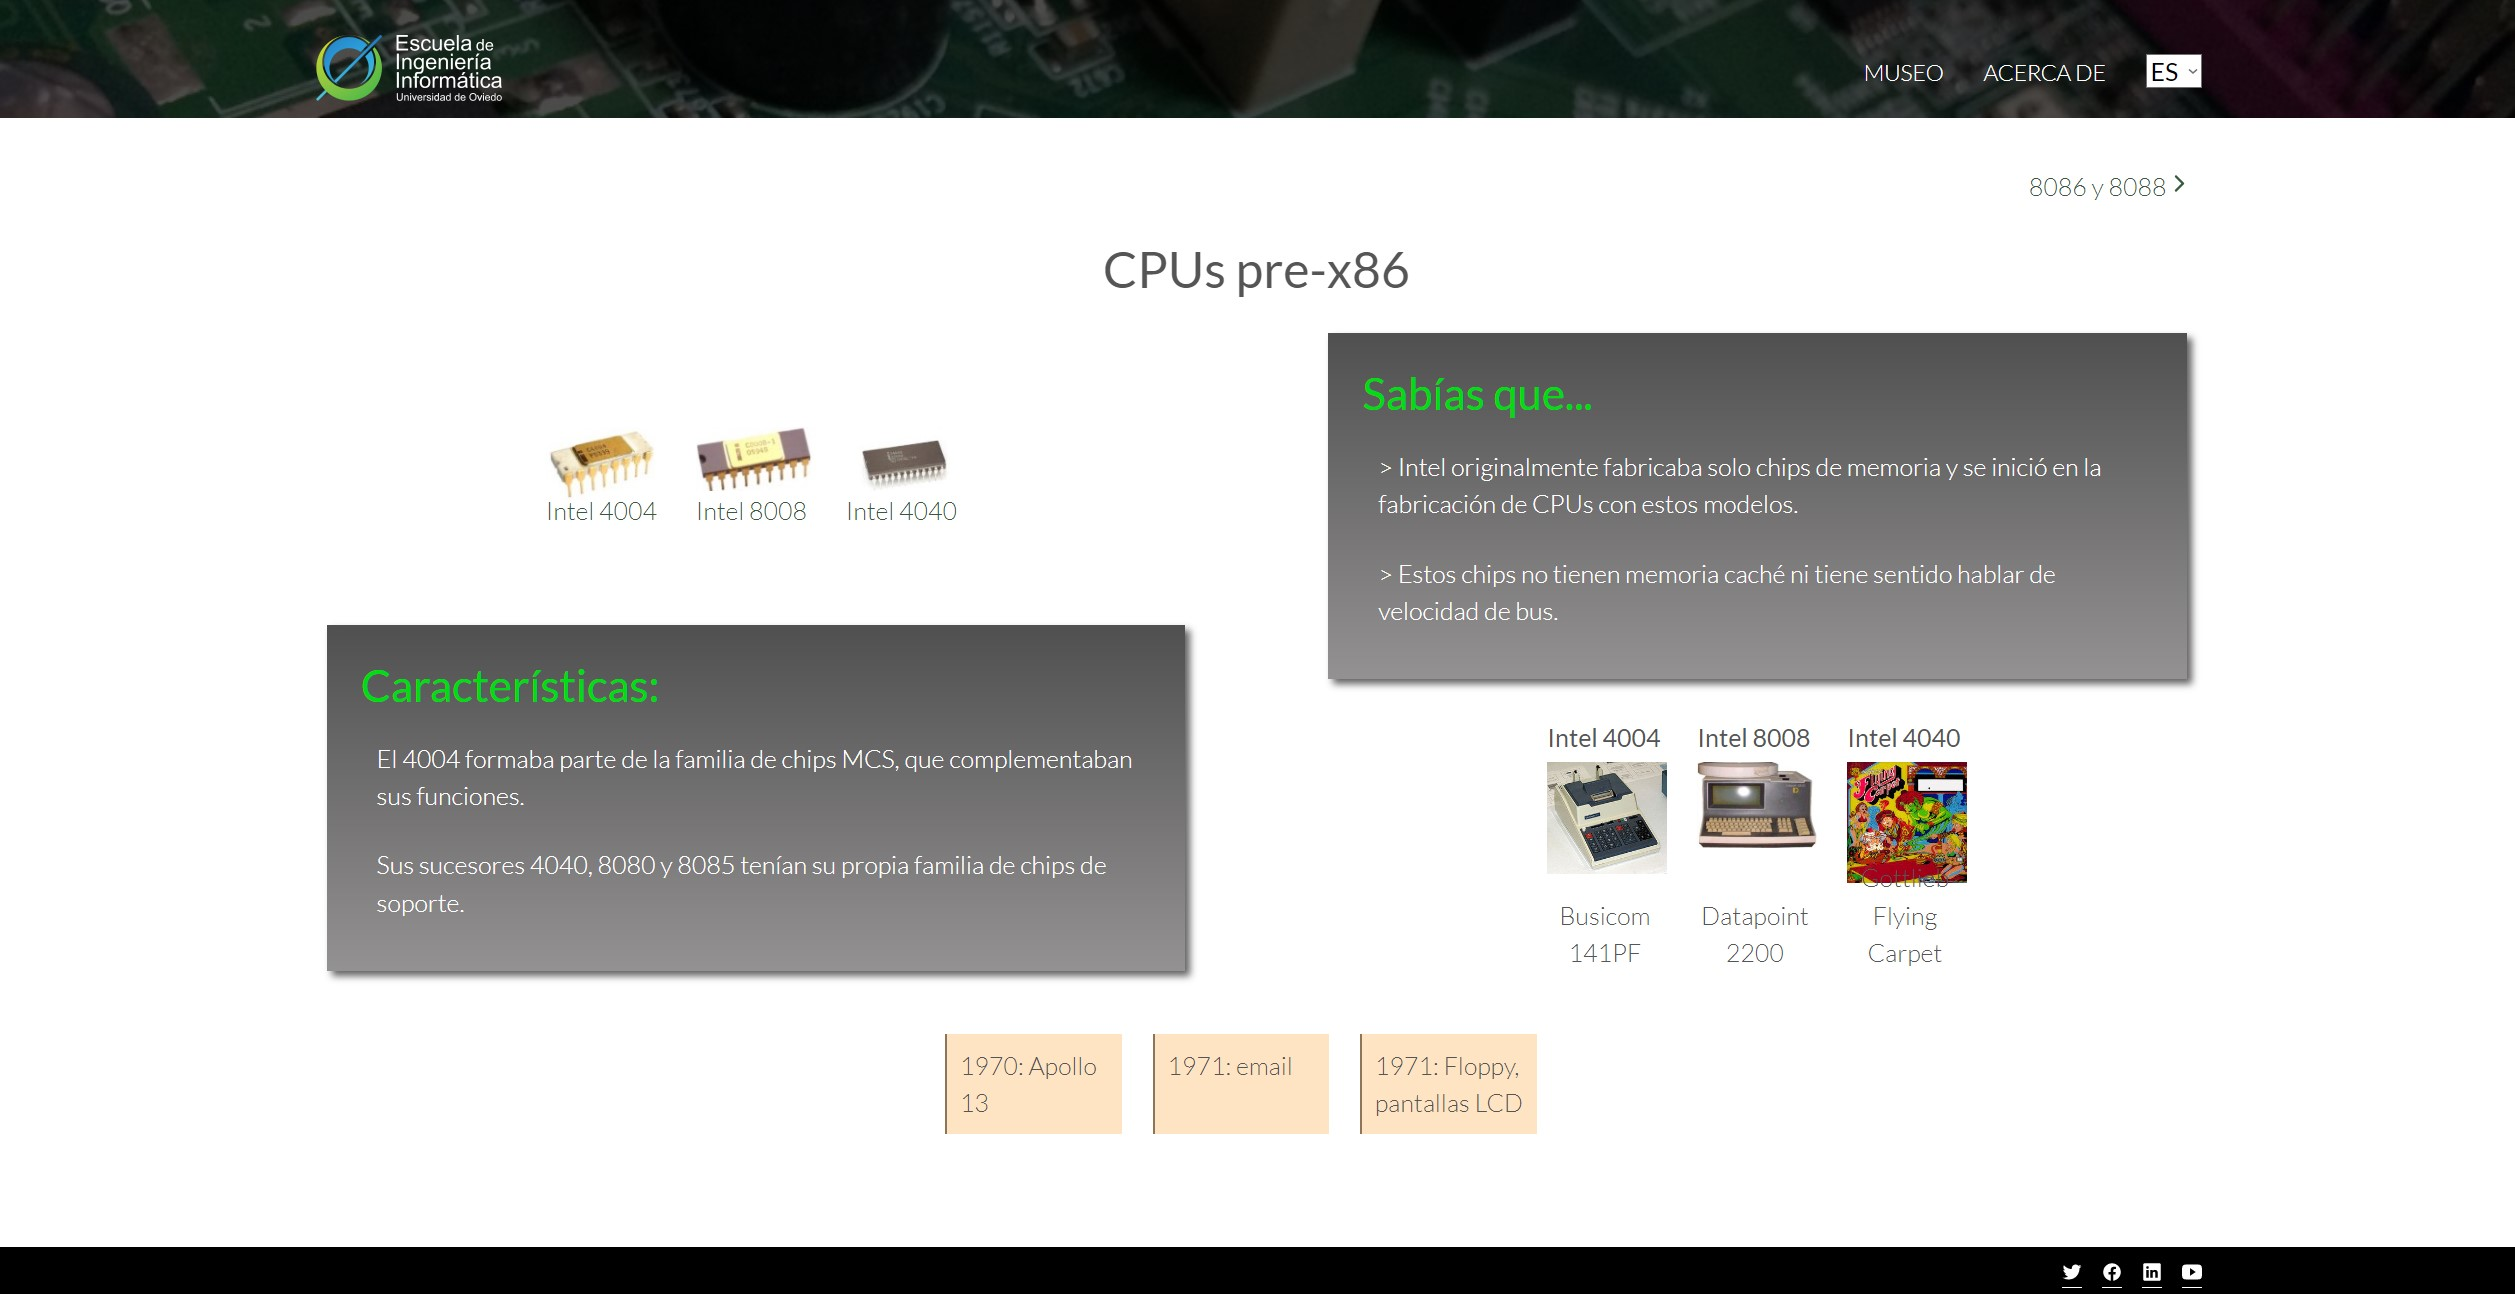
\includegraphics[scale=0.25]{periodoIUDef}
%\caption{Página de detalles del periodo (museo)}
%\end{figure}
%\begin{figure}[H]
%\centering
%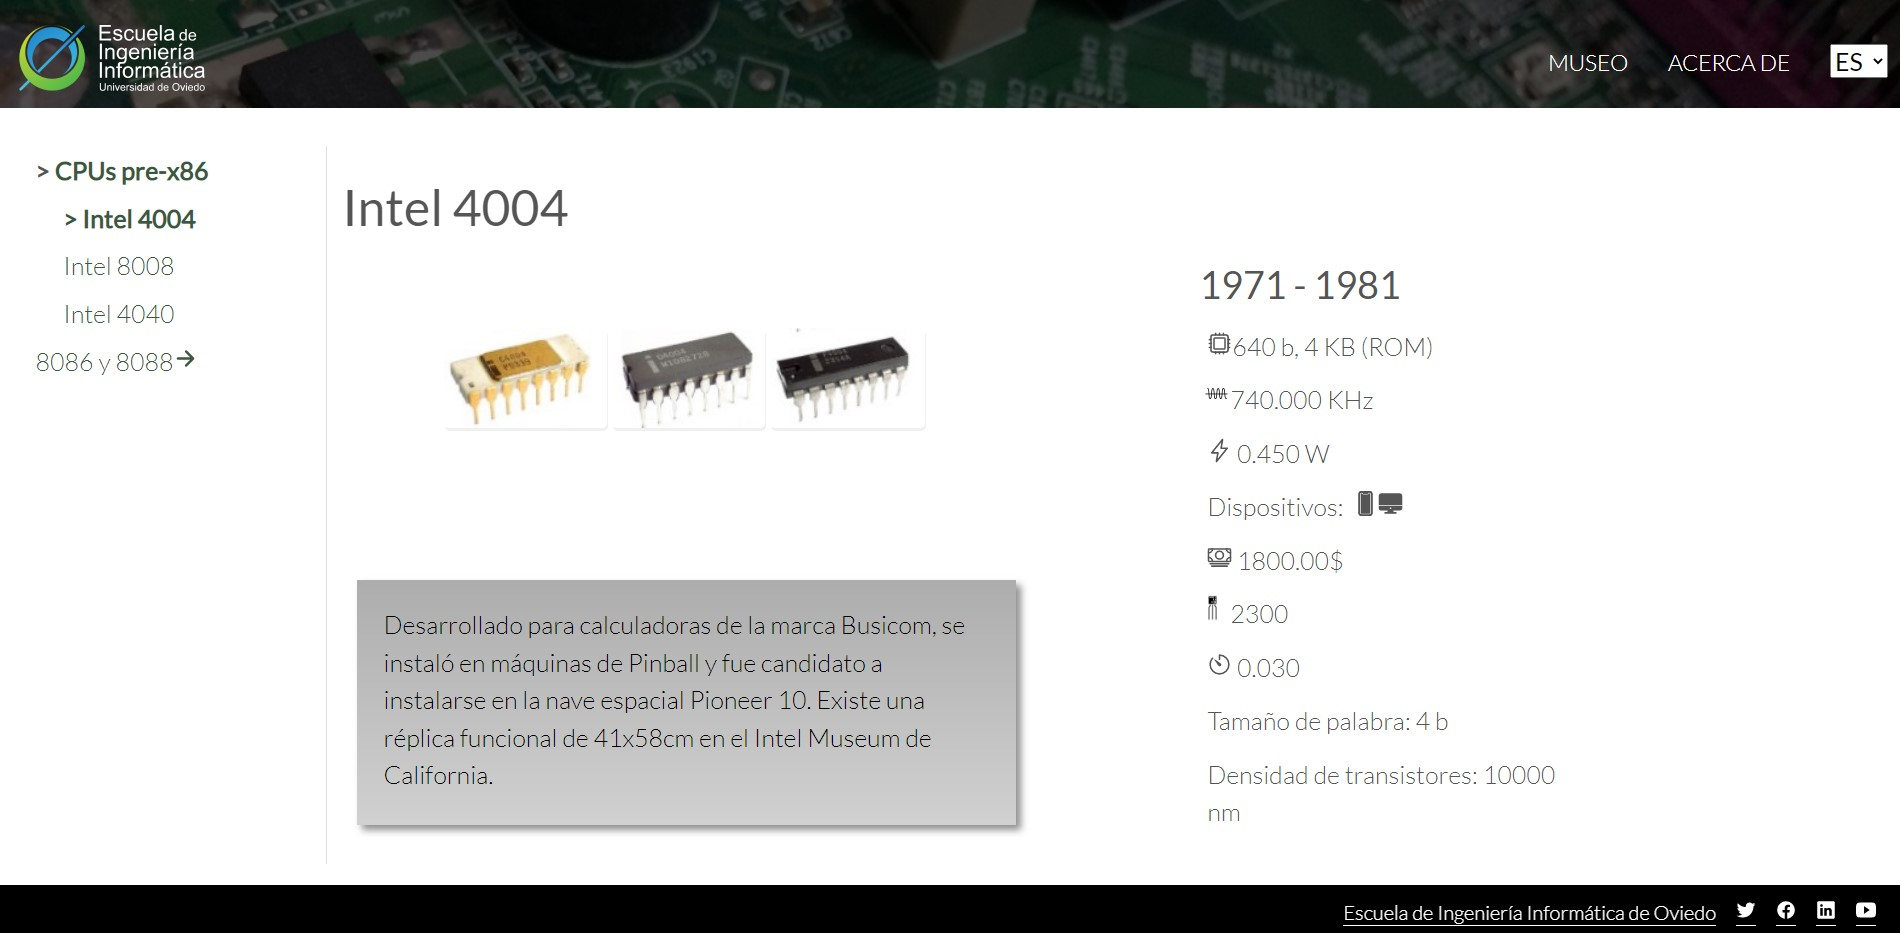
\includegraphics[scale=0.25]{piezaIUDef}
%\caption{Página de detalles del componente (museo)}
%\end{figure}
%
%\subsubsection{Administración del museo}
%\begin{figure}[H]
%\centering
%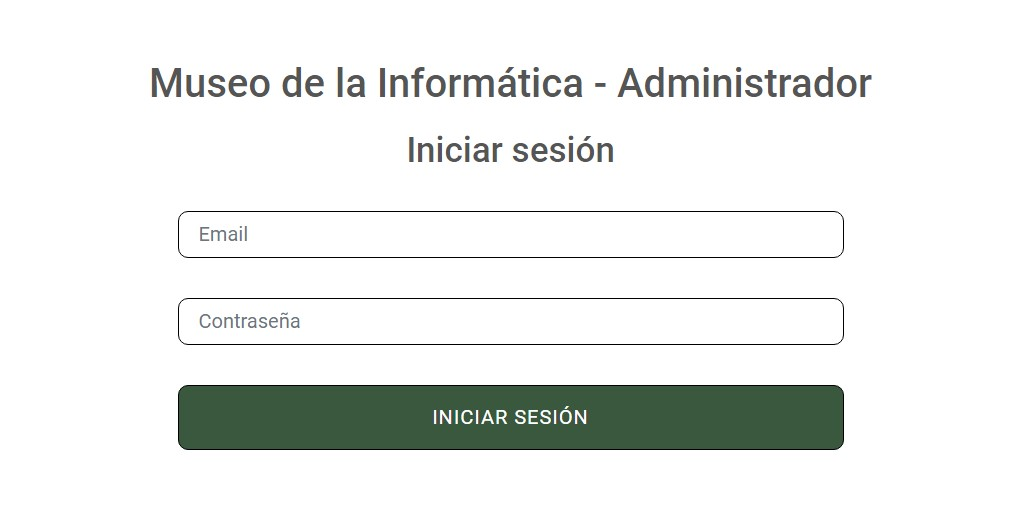
\includegraphics[scale=0.55]{loginIUDef}
%\caption{Página de inicio de sesión}
%\end{figure}
%\begin{figure}[H]
%\centering
%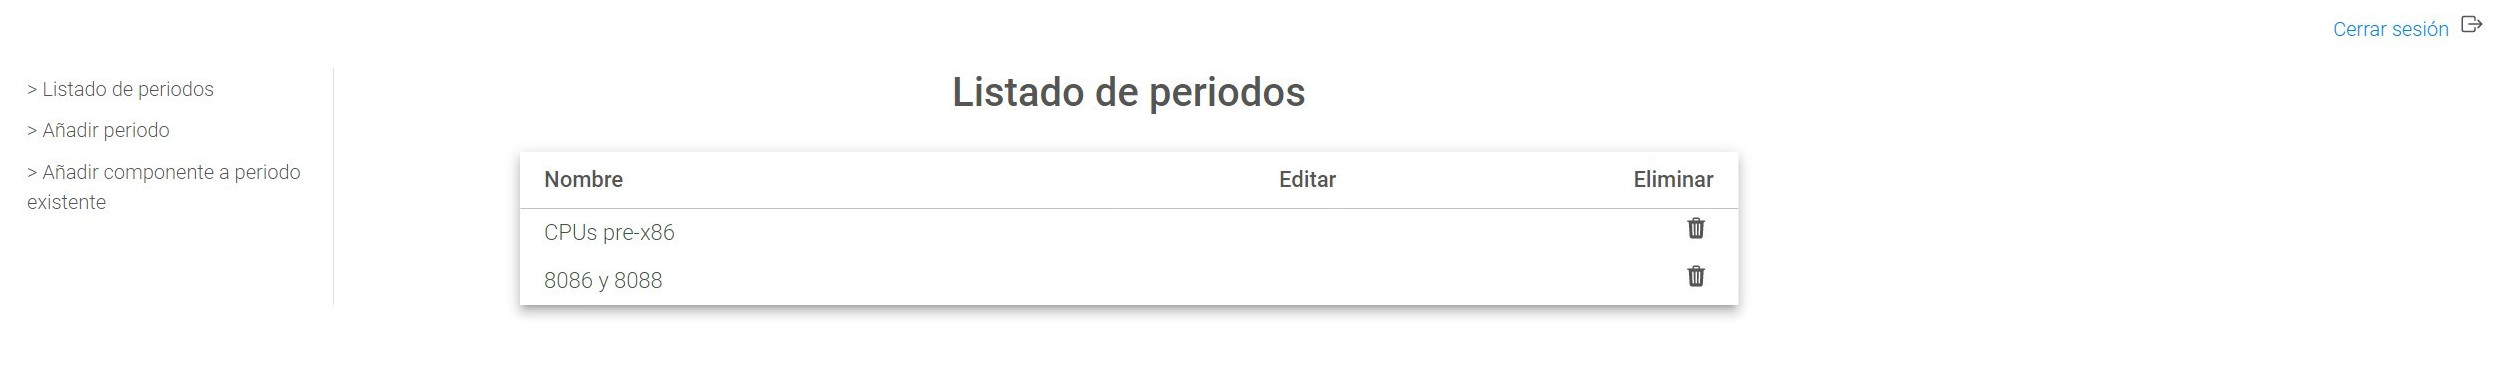
\includegraphics[scale=0.35]{listadoPeriodosIUDef}
%\caption{Página de listado de periodos}
%\end{figure}
%\begin{figure}[H]
%\centering
%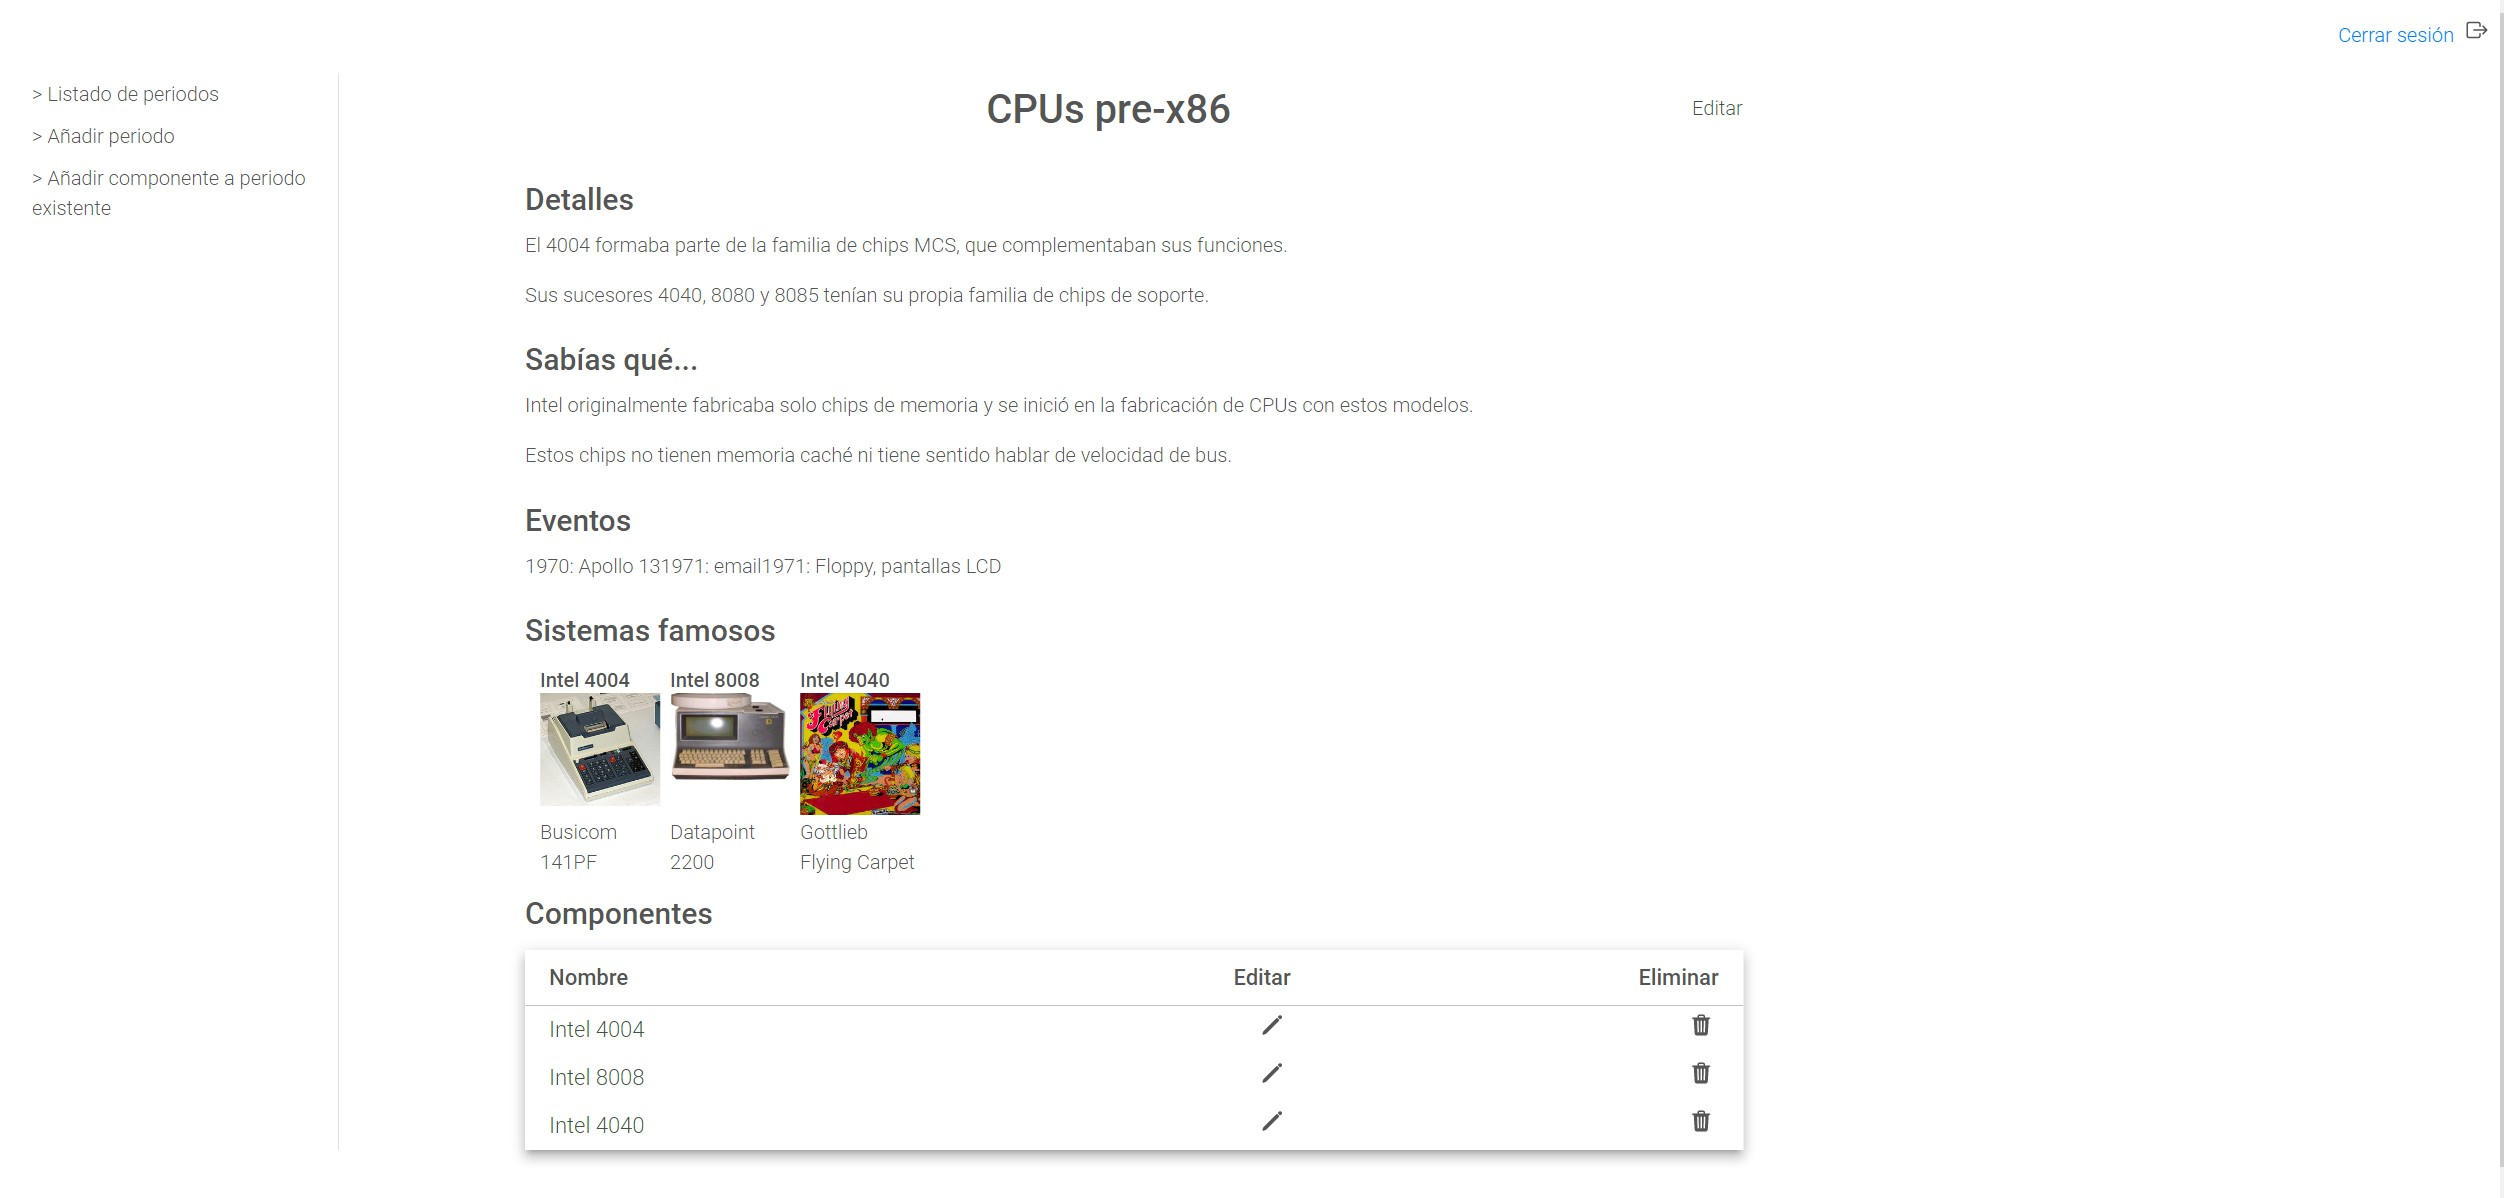
\includegraphics[scale=0.35]{periodoIU2Def}
%\caption{Página de detalles de un periodo (administración)}
%\end{figure}
%\begin{figure}[H]
%\centering
%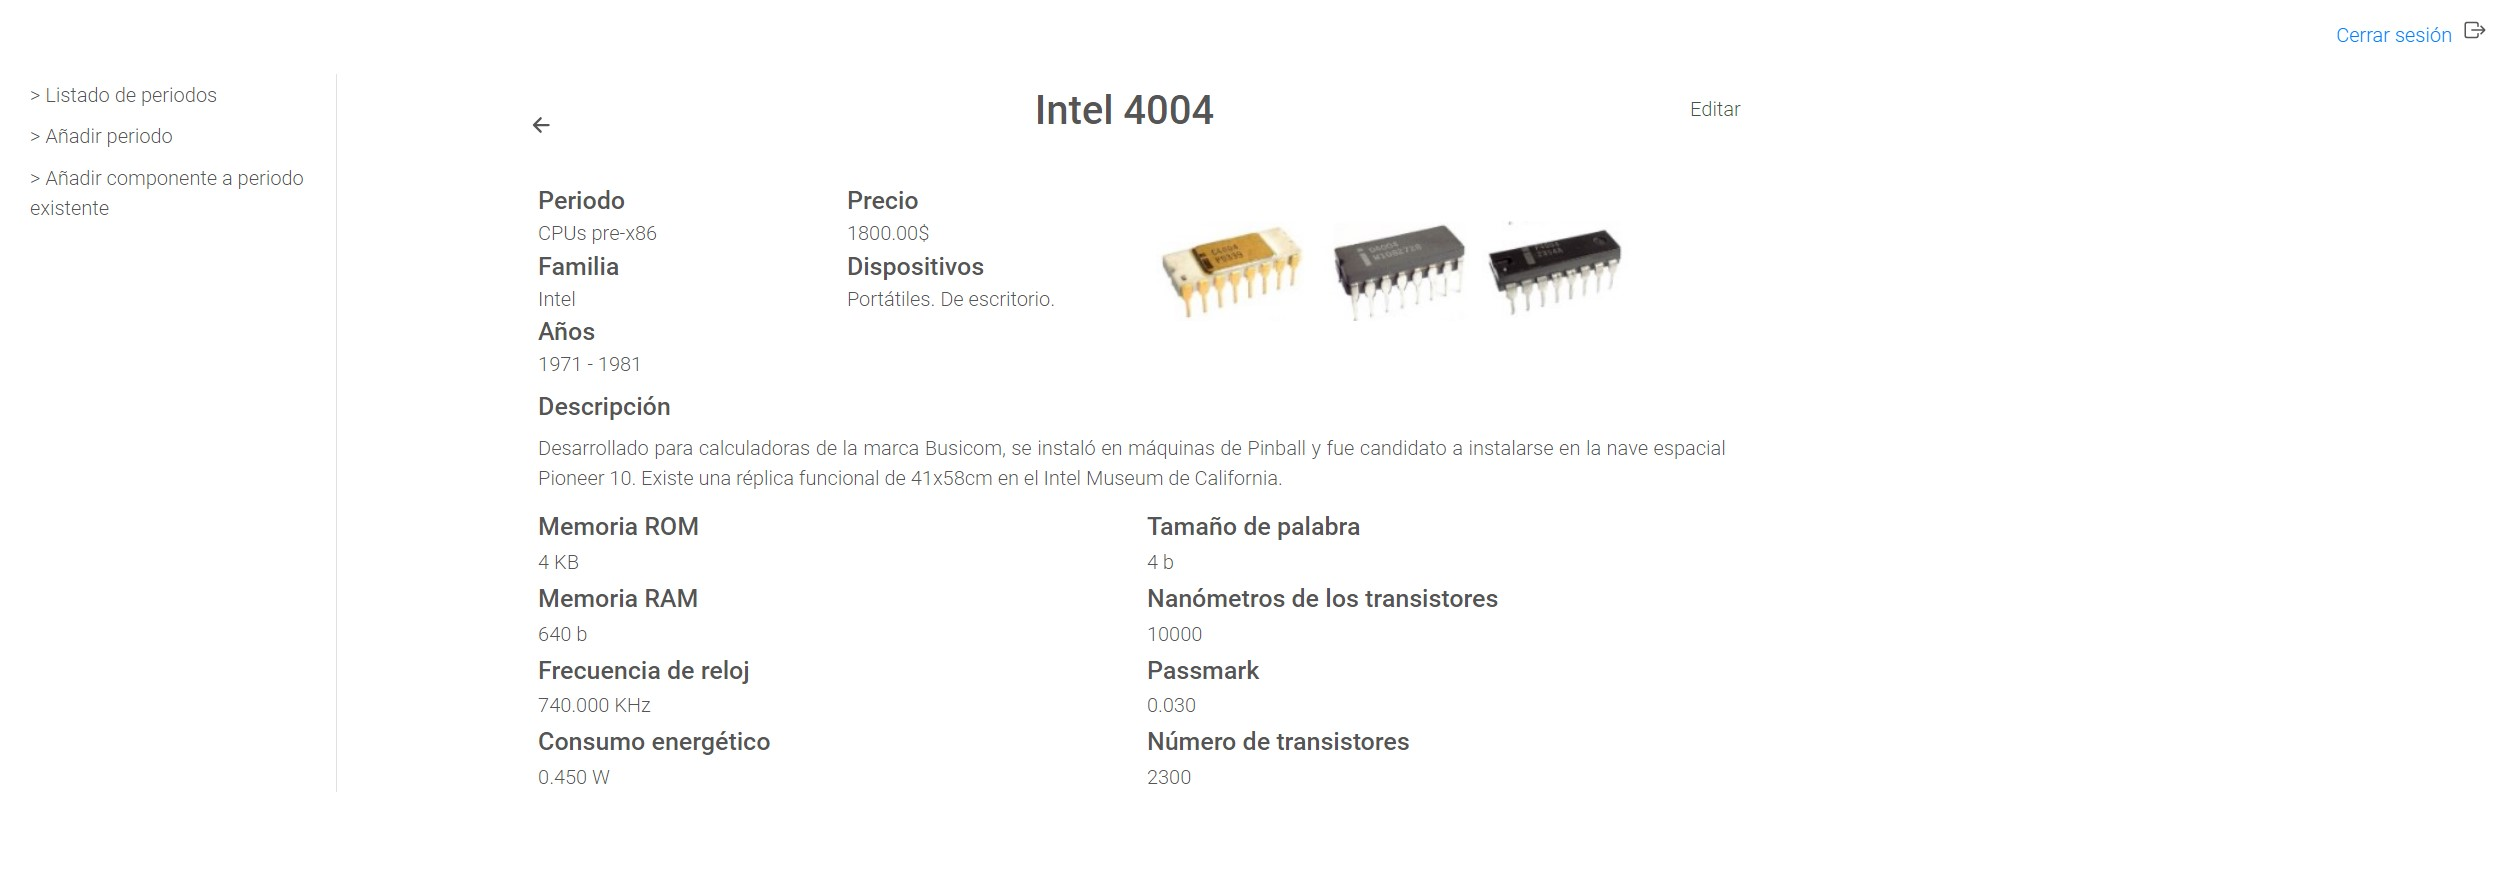
\includegraphics[scale=0.35]{compIUDef}
%\caption{Página de detalles de un componente (administración)}
%\end{figure}
%\begin{figure}[H]
%\centering
%\includegraphics[scale=0.35]{añadirPeriodoIUDef}
%\caption{Formulario para añadir un periodo}
%\end{figure}
%\begin{figure}[H]
%\centering
%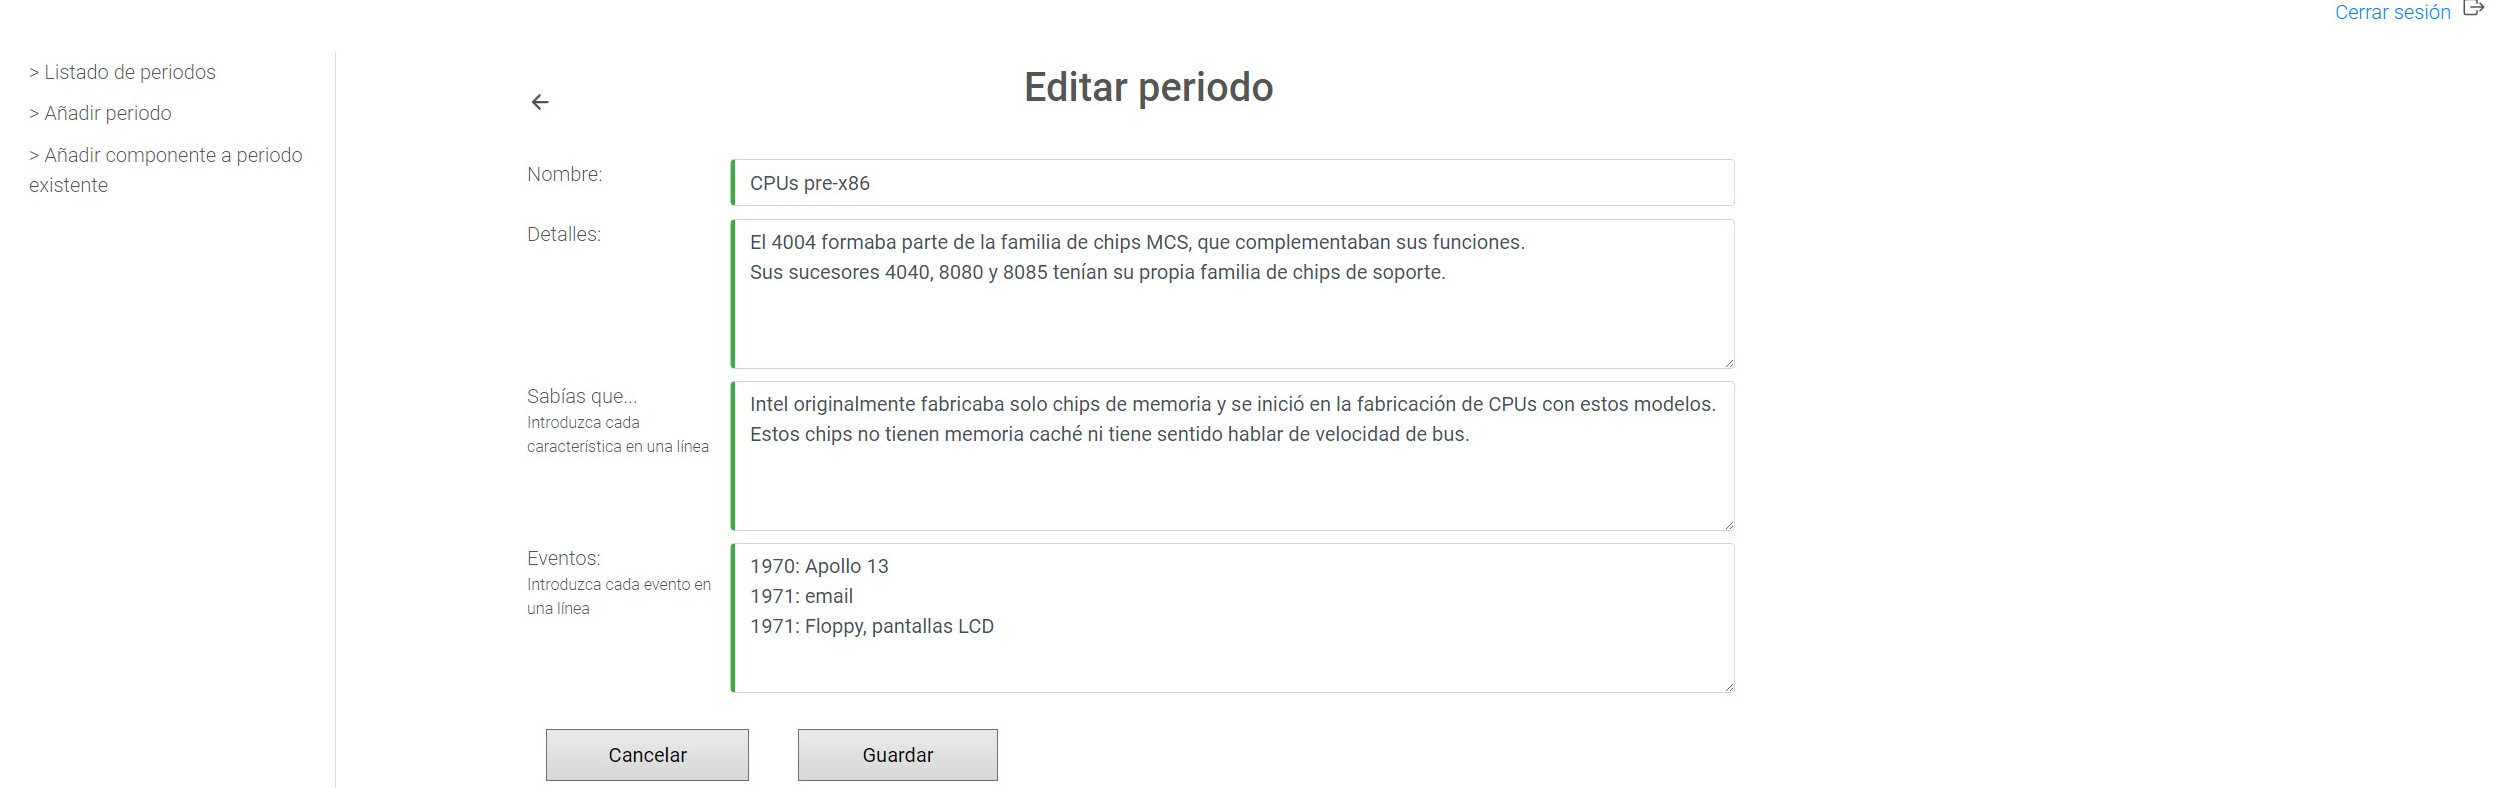
\includegraphics[scale=0.35]{editarPeriodoIUDef}
%\caption{Formulario para editar un periodo}
%\end{figure}
%\begin{figure}[H]
%\centering
%\includegraphics[scale=0.35]{añadirCompIUDef}
%\caption{Formulario para añadir un componente}
%\end{figure}
%\begin{figure}[H]
%\centering
%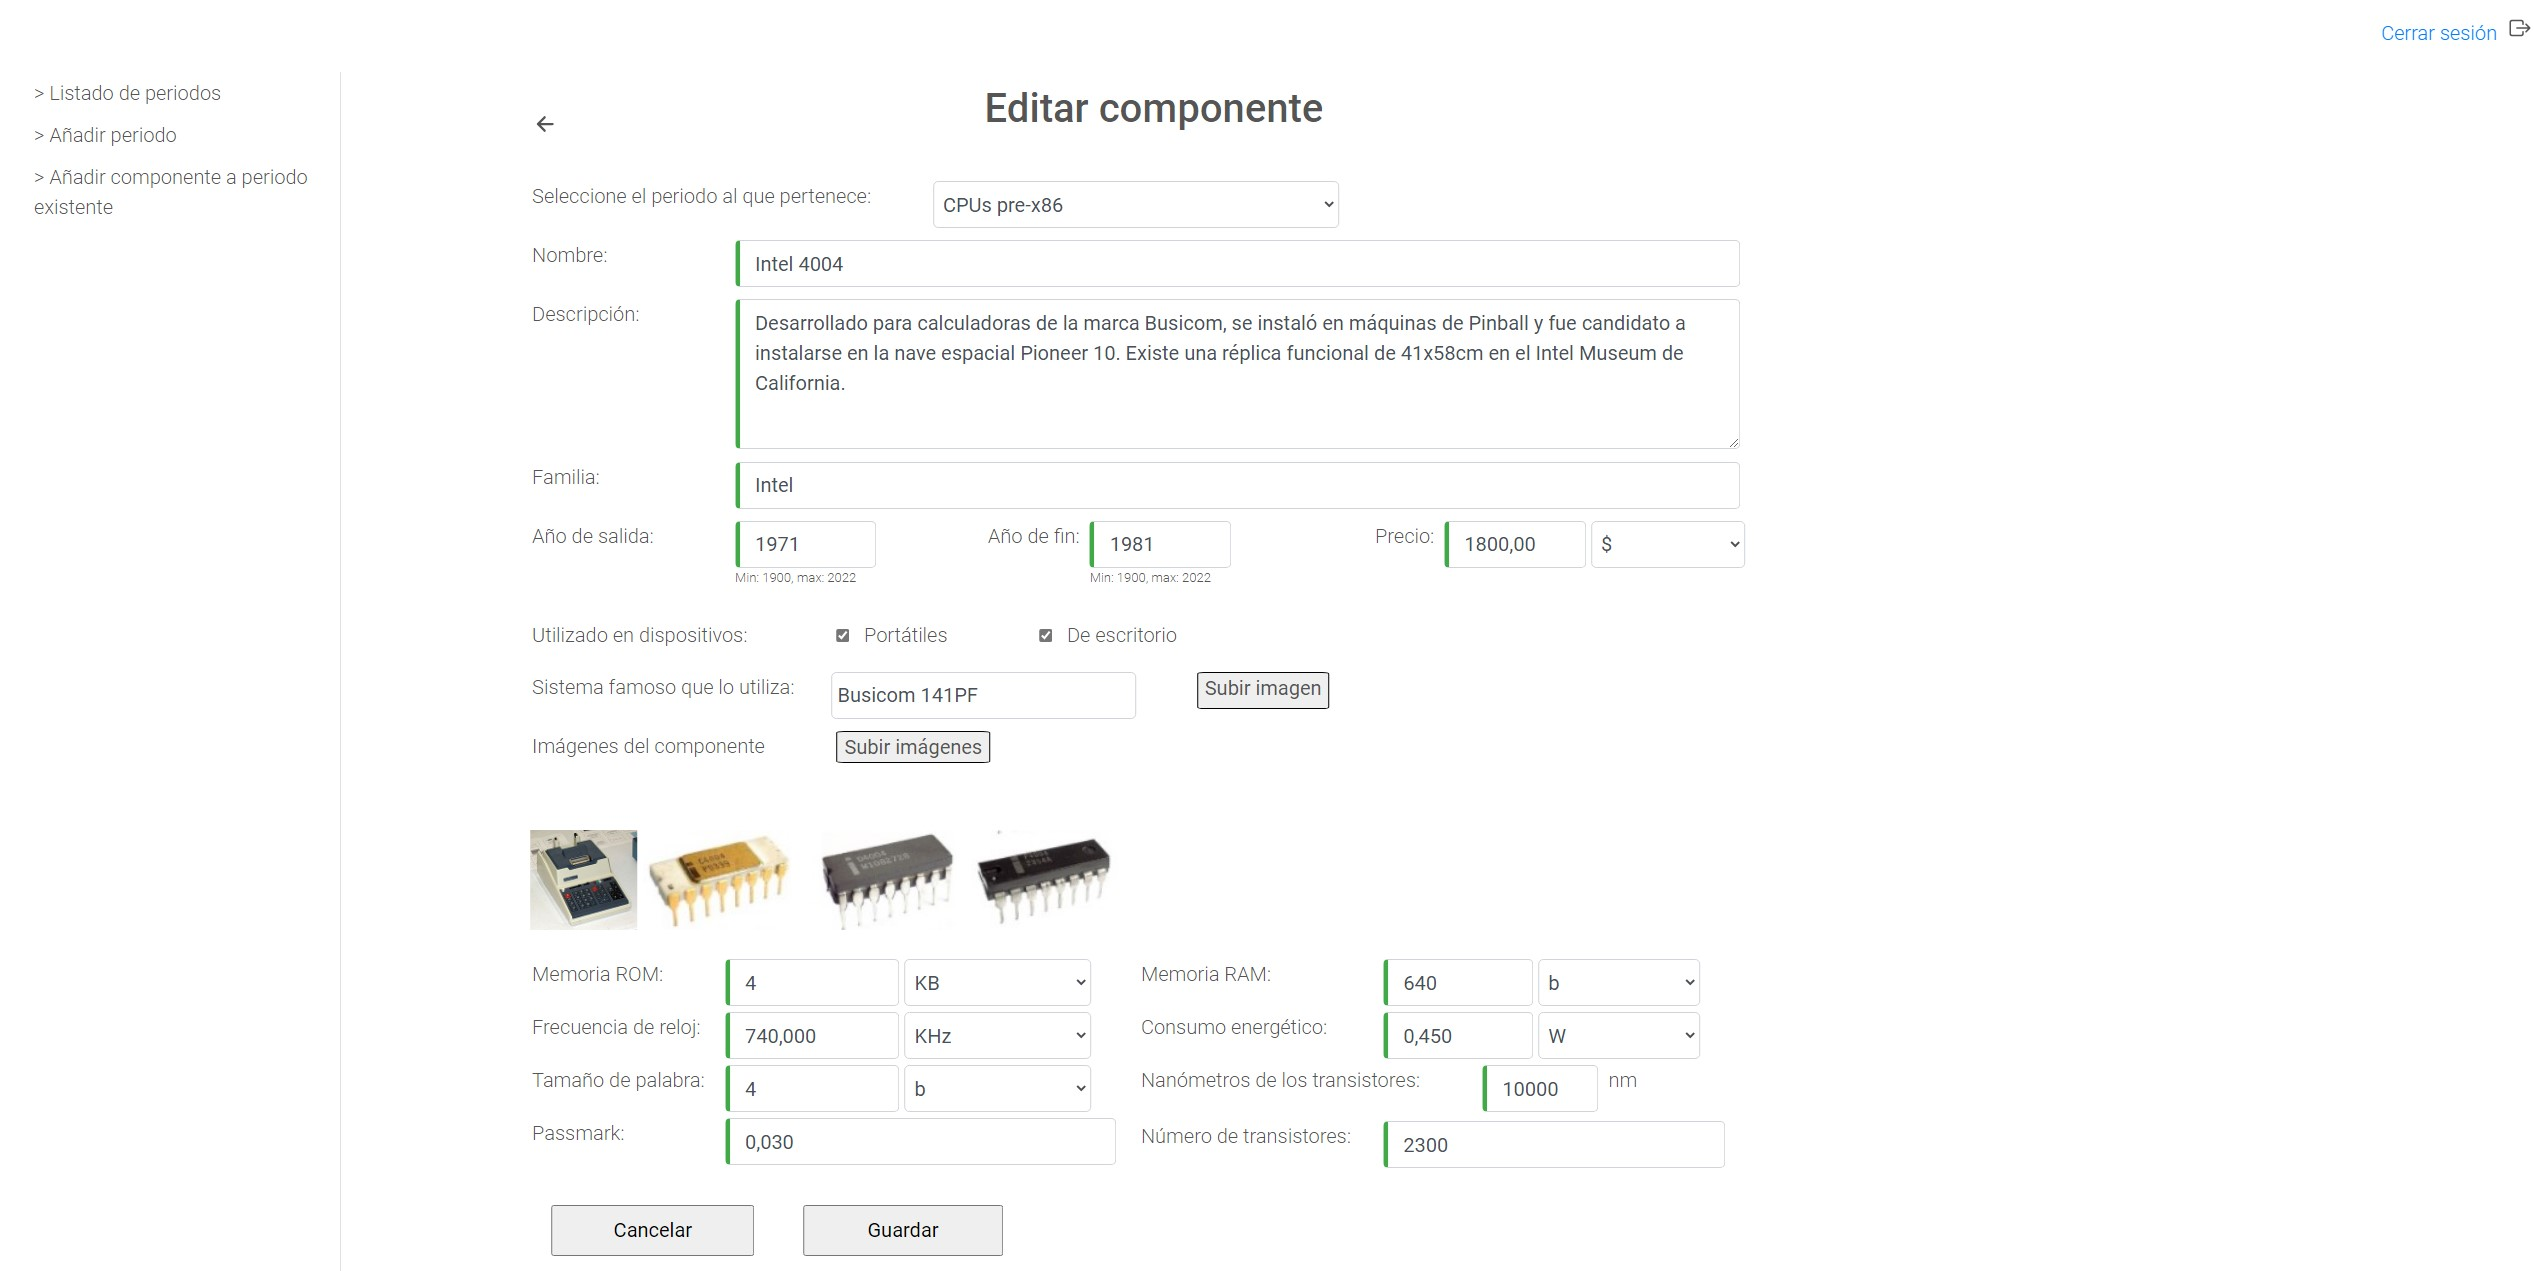
\includegraphics[scale=0.35]{editarCompIUDef}
%\caption{Formulario para editar un componente}
%\end{figure}


%\newpage
%\section{DSI 9: DISEÑO DE LA MIGRACIÓN Y CARGA INICIAL DE DATOS}


\newpage
\section{DSI 10: ESPECIFICACIÓN TÉCNICA DEL PLAN DE PRUEBAS}

\subsection{Pruebas Unitarias y del Sistema} 

\begin{table}[H]
%\vspace{-4mm}
  \centering
  \caption{Diseño de pruebas: Consultar periodos (museo)}
    \begin{tabular}{p{9em}p{12em}p{15em}}
    \toprule
    \rowcolor[rgb]{ .851,  .886,  .953} \multicolumn{3}{p{36em}}{\textbf{Consultar periodos (museo)}} \\ \midrule
    \rowcolor[rgb]{ .949,  .949,  .949} \textbf{Prueba} & \textbf{Pasos} & \textbf{Resultado esperado}\\ \midrule
    \textbf{Obtener periodos existentes} & - Acceder a la vista general del museo & El sistema devolverá una lista de todos los periodos existentes. \\ \midrule
    \textbf{Obtener periodo por nombre} & - Acceder a la vista general del museo.\par - Introducir un texto en la barra de búsqueda. & El sistema devolverá una lista de los periodos cuyo nombre contenga el texto introducido. \\ \midrule
    \textbf{Obtener periodo por años} & - Acceder a la vista general del museo.\par - Cambiar los años especificados en la barra deslizadora. & El sistema devolverá una lista de los periodos cuyos años coincidan con los introducidos.\\ \bottomrule
    \end{tabular}%
\end{table}%
\begin{table}[H]
\vspace{-4mm}
  \centering
  \caption{Diseño de pruebas: Consultar componentes (museo)}
    \begin{tabular}{p{11em}p{11em}p{14em}}
    \toprule
    \rowcolor[rgb]{ .851,  .886,  .953} \multicolumn{3}{p{36em}}{\textbf{Consultar componentes (museo)}} \\ \midrule
    \rowcolor[rgb]{ .949,  .949,  .949} \textbf{Prueba} & \textbf{Pasos} & \textbf{Resultado esperado}\\ \midrule
    \textbf{Obtener componentes de un periodo} & - Acceder a un periodo. & El sistema devolverá una lista de todos los componentes pertenecientes al periodo. \\ \bottomrule
    \end{tabular}%
\end{table}%
\begin{table}[H]
\vspace{-4mm}
  \centering
  \caption{Diseño de pruebas: Iniciar sesión}
    \begin{tabular}{p{9em}p{11em}p{16em}}
    \toprule
    \rowcolor[rgb]{ .851,  .886,  .953} \multicolumn{3}{p{36em}}{\textbf{Iniciar sesión}} \\ \midrule
    \rowcolor[rgb]{ .949,  .949,  .949} \textbf{Prueba} & \textbf{Pasos} & \textbf{Resultado esperado}\\ \midrule
    \textbf{Iniciar sesión con datos válidos } & - Introducir el usuario \textit{uo257829@uniovi.es}.\par - Introducir la contraseña \textit{museoinfo2022}. & El sistema permitirá el acceso a la página de administración. \\ \midrule
    \textbf{Iniciar sesión con datos incorrectos} & - Introducir el usuario \textit{uo257829@uniovi.es}.\par - Introducir la contraseña \textit{123456}. & El sistema no permitirá el acceso y se mostrará un error. \\ \bottomrule
    \end{tabular}%
\end{table}%
\begin{table}[H]
\vspace{-4mm}
  \centering
  \caption{Diseño de pruebas: Consultar periodos (administración)}
    \begin{tabular}{p{9em}p{11em}p{16em}}
    \toprule
    \rowcolor[rgb]{ .851,  .886,  .953} \multicolumn{3}{p{36em}}{\textbf{Consultar periodos (administración)}} \\ \midrule
    \rowcolor[rgb]{ .949,  .949,  .949} \textbf{Prueba} & \textbf{Pasos} & \textbf{Resultado esperado}\\ \midrule
    \textbf{Obtener periodos existentes} & - Acceder al listado de periodos. & El sistema devolverá una lista de todos los periodos existentes. \\ \bottomrule
    \end{tabular}%
\end{table}%
\begin{table}[H]
\vspace{-4mm}
  \centering
  \caption{Diseño de pruebas: Añadir periodo}
    \begin{tabular}{p{8em}p{14em}p{14em}}
    \toprule
    \rowcolor[rgb]{ .851,  .886,  .953} \multicolumn{3}{p{36em}}{\textbf{Añadir periodo}} \\ \midrule
    \rowcolor[rgb]{ .949,  .949,  .949} \textbf{Prueba} & \textbf{Pasos} & \textbf{Resultado esperado}\\ \midrule
    \textbf{Añadir nuevo periodo (periodo 2)} & - Acceder a añadir un periodo.\par - Introducir los datos \textit{Periodo 2, detalles, eventos, curiosidades}. \par - Guardar periodo. & El sistema tendrá un periodo más. \\ \midrule
    \textbf{Añadir periodo que ya existe (periodo 1)} & - Acceder a añadir un periodo.\par - Introducir los datos \textit{Periodo 1, detalles, eventos, curiosidades}. \par - Guardar periodo. & El sistema no añadirá el periodo y responderá con un error.  \\ \midrule
    \textbf{Añadir periodo con campos vacíos} &  - Acceder a añadir un periodo.\par - Introducir los datos \textit{Periodo 2, ' ', eventos, curiosidades}. \par - Guardar periodo. & El sistema no añadirá el periodo y responderá con un error. \\ \bottomrule
    \end{tabular}%
\end{table}%
\begin{table}[H]
\vspace{-4mm}
  \centering
  \caption{Diseño de pruebas: Modificar periodo}
    \begin{tabular}{p{10em}p{13em}p{14em}}
    \toprule
    \rowcolor[rgb]{ .851,  .886,  .953} \multicolumn{3}{p{36em}}{\textbf{Modificar periodo}} \\ \midrule
    \rowcolor[rgb]{ .949,  .949,  .949} \textbf{Prueba} & \textbf{Entrada} & \textbf{Resultado esperado}\\ \midrule
    \textbf{Modificar periodo existente (periodo 1)} & - Introducir los datos \textit{Periodo 1 modificado, detalles, eventos, curiosidades, 1}.\par - Guardar periodo. & El sistema actualizará los datos del periodo. \\ \midrule
    \textbf{Modificar un periodo que no existe (periodo 25)} & - Introducir los datos \textit{Periodo 25 modificado, detalles, eventos, curiosidades, 25}.\par - Guardar periodo. & El sistemá responderá con un error. \\ \midrule
    \textbf{Modificar periodo dejando campos vacíos} & - Introducir los datos \textit{Periodo 1 modificado, detalles, eventos, ' ', 1}.\par - Guardar periodo. & El sistema no actualizará el periodo y responderá con un error. \\ \bottomrule
    \end{tabular}%
\end{table}%
\begin{table}[H]
\vspace{-4mm}
  \centering
  \caption{Diseño de pruebas: Eliminar periodo}
    \begin{tabular}{p{11em}p{11em}p{14em}}
    \toprule
    \rowcolor[rgb]{ .851,  .886,  .953} \multicolumn{3}{p{36em}}{\textbf{Eliminar periodo}} \\ \midrule
    \rowcolor[rgb]{ .949,  .949,  .949} \textbf{Prueba} & \textbf{Entrada} & \textbf{Resultado esperado}\\ \midrule
    \textbf{Eliminar un periodo existente (periodo 1)} & - Eliminar periodo 1.  & El sistema tendrá un periodo menos. \\ \midrule
    \textbf{Eliminar un periodo que no existe (periodo 25)} & - Eliminar periodo 25.  & El sistema responderá con un error. \\ \bottomrule
    \end{tabular}%
\end{table}%
\begin{table}[H]
\vspace{-4mm}
  \centering
  \caption{Diseño de pruebas: Consultar componentes (administración)}
    \begin{tabular}{p{11em}p{11em}p{14em}}
    \toprule
    \rowcolor[rgb]{ .851,  .886,  .953} \multicolumn{3}{p{36em}}{\textbf{Consultar componentes (administración)}} \\ \midrule
    \rowcolor[rgb]{ .949,  .949,  .949} \textbf{Prueba} & \textbf{Entrada} & \textbf{Resultado esperado}\\ \midrule
    \textbf{Obtener componentes de un periodo} & - Acceder a un periodo. & El sistema devolverá una lista de todos los componentes pertenecientes al periodo. \\ \bottomrule
    \end{tabular}%
\end{table}%
\begin{table}[H]
\vspace{-4mm}
  \centering
  \caption{Diseño de pruebas: Añadir componente}
    \begin{tabular}{p{13em}p{15em}p{8em}}
    \toprule
    \rowcolor[rgb]{ .851,  .886,  .953} \multicolumn{3}{p{36em}}{\textbf{Añadir componente}} \\ \midrule
    \rowcolor[rgb]{ .949,  .949,  .949} \textbf{Prueba} & \textbf{Entrada} & \textbf{Resultado esperado}\\ \midrule
    \textbf{Añadir nuevo componente (CPU 2)} & - Acceder a añadir componente. \par - Introducir los datos \textit{CPU 2, familia, descripción, años, periodo 1, etc.}\par - Guardar componente. & El sistema tendrá un componente más. \\ \midrule
    \textbf{Añadir componente que ya existe (CPU 1)} & - Acceder a añadir componente. \par - Introducir los datos \textit{CPU 1, familia, descripción, años, periodo 1, etc.}\par - Guardar componente.  & El sistema no añadirá el componente y responderá con un error.  \\ \midrule
    \textbf{Añadir componente a un periodo que no existe (CPU 3, periodo 25)} & - Acceder a añadir componente. \par - Introducir los datos \textit{CPU 3, familia, descripción, años, periodo 25, etc.}\par - Guardar componente.  & El sistema no añadirá el componente y responderá con un error.  \\ \midrule
    \textbf{Añadir componente con campos obligatorios vacíos} & - Acceder a añadir componente. \par - Introducir los datos \textit{CPU 3, familia, ' ', años, perido 1, etc.}\par - Guardar componente.  & El sistema no añadirá el componente y responderá con un error. \\ \bottomrule
    \end{tabular}%
\end{table}%
\begin{table}[H]
\vspace{-4mm}
  \centering
  \caption{Diseño de pruebas: Modificar componente}
    \begin{tabular}{p{13em}p{11em}p{12em}}
    \toprule
    \rowcolor[rgb]{ .851,  .886,  .953} \multicolumn{3}{p{36em}}{\textbf{Modificar componente}} \\ \midrule
    \rowcolor[rgb]{ .949,  .949,  .949} \textbf{Prueba} & \textbf{Entrada} & \textbf{Resultado esperado}\\ \midrule
    \textbf{Modificar componente existente (CPU 1)} & - Introducir los datos \textit{CPU 1 modificada, familia, descripción, años, periodo 1, 1, etc.}\par - Guardar componente. & El sistema actualizará los datos del componente. \\ \midrule
    \textbf{Modificar un componente que no existe (CPU 30)} & - Introducir los datos \textit{CPU 30 modificada, familia, descripción, años, periodo 1, 30, etc.}\par - Guardar componente. & El sistemá responderá con un error. \\ \midrule
    \textbf{Modificar componente dejando campos obligatorios vacíos} & - Introducir los datos \textit{CPU 1 modificada, familia, ' ', años, periodo 1, 1, etc.}\par - Guardar componente. & El sistema no actualizará el componente y responderá con un error. \\ \bottomrule
    \end{tabular}%
\end{table}%
\begin{table}[H]
\vspace{-4mm}
  \centering
  \caption{Diseño de pruebas: Eliminar componente}
    \begin{tabular}{p{13em}p{11em}p{12em}}
    \toprule
    \rowcolor[rgb]{ .851,  .886,  .953} \multicolumn{3}{p{36em}}{\textbf{Eliminar componente}} \\ \midrule
    \rowcolor[rgb]{ .949,  .949,  .949} \textbf{Prueba} & \textbf{Entrada} & \textbf{Resultado esperado}\\ \midrule
    \textbf{Eliminar un componente existente (CPU 1)} & - Eliminar CPU 1. & El sistema tendrá un componente menos. \\ \midrule
    \textbf{Eliminar un componente que no existe (CPU 30)} & - Eliminar CPU 30. & El sistema responderá con un error. \\ \bottomrule
    \end{tabular}%
\end{table}%


\subsection{Pruebas de Usabilidad y Accesibilidad} 
Las pruebas de usabilidad y accesibilidad de la aplicación web del museo serán realizadas por usuarios con distintos perfiles, mientras que las de la aplicación de administración solo las realizará el usuario administrador, ya que será el único que interactúe con este sistema. Los usuarios interactuarán con el sistema y rellenarán un cuestionario, que será detallado a continuación. También habrá un cuestionario en el que el responsable de las pruebas anotará las observaciones realizadas durante las pruebas.

\subsubsection{Cuestionario de evaluación} 
\paragraph*{Preguntas de carácter general}
\begin{table}[H]
\centering
\caption{Pruebas de usabilidad: preguntas de carácter general}
\begin{tabular}{p{36em}}
\toprule
\rowcolor[rgb]{ .949,  .949,  .949} \textbf{¿Usa un ordenador frecuentemente?} \\ \midrule
\vspace{-4mm}
\begin{enumerate}
\item Todos los días
\item Varias veces a la semana
\item Ocasionalmente
\item Nunca
\end{enumerate} \\ \midrule
\rowcolor[rgb]{ .949,  .949,  .949} \textbf{¿Qué tipo de actividades realiza con el ordenador?} \\ \midrule
\vspace{-4mm}
\begin{enumerate}
\item Es parte de mi trabajo o profesión
\item Lo uso básicamente para ocio
\item Solo empleo aplicaciones estilo Office
\item Únicamente leo el correo y navego ocasionalmente
\end{enumerate} \\ \midrule
\rowcolor[rgb]{ .949,  .949,  .949} \textbf{¿Qué busca Vd. principalmente en una aplicación web?} \\ \midrule
\vspace{-4mm}
\begin{enumerate}
\item Que sea fácil de navegar
\item Que sea intuitiva
\item Que sea rápida
\end{enumerate} \\ \bottomrule
\end{tabular}
\end{table}

\paragraph*{Actividades guiadas}
Las actividades que realizarán los diferentes usuarios en la aplicación web del museo son las siguientes:
\begin{itemize}
\item Navegar por la linea temporal presente en la vista general del museo.
\item Realizar una búsqueda por años.
\item Realizar una búsqueda por nombre.
\item Consultar los detalles de un periodo.
\item Consultar los detalles de un componente.
\end{itemize}
El administrador realizará las actividades mencionadas y también las correspondientes a la aplicación de administración, que se muestran a continuación:
\begin{itemize}
\item Añadir un periodo.
\item Añadir un componente.
\item Editar un periodo.
\item Editar un componente.
\item Eliminar un periodo.
\item Eliminar un componente.
\end{itemize}

\paragraph*{Preguntas cortas sobre la aplicación y observaciones}
\begin{table}[H]
\centering
\caption{Pruebas de usabilidad: preguntas sobre la aplicación}
\begin{tabular}{p{15em}|p{4em}|p{7.5em}|p{7.5em}|p{3em}}
\toprule
\rowcolor[rgb]{.949,  .949,  .949} \textbf{Facilidad de uso} & \textbf{Siempre} & \textbf{Frecuentemente} & \textbf{Ocasionalmente} & \textbf{Nunca} \\ \midrule
\textit{¿Sabe dónde está dentro de la aplicación?} & & & & \\ \midrule
\textit{¿Necesita ayuda para utilizar la aplicación?} & & & & \\ \midrule
\textit{¿Le resulta sencillo el uso de la aplicación?} & & & & \\ \midrule
\textit{¿Identifica fácilmente la información que se le presenta?} & & & & \\ \midrule
\rowcolor[rgb]{.949,  .949,  .949} \textbf{Funcionalidad} & \textbf{Siempre} & \textbf{Frecuentemente} & \textbf{Ocasionalmente} & \textbf{Nunca} \\ \midrule
\textit{¿Funciona cada tarea como Vd. espera?} & & & & \\ \midrule
\textit{¿El tiempo de respuesta de la aplicación es muy grande?} & & & & \\ \midrule
\rowcolor[rgb]{ .851,  .886,  .953} \multicolumn{5}{p{36em}}{\textbf{Calidad del interfaz}} \\ \midrule
\rowcolor[rgb]{.949,  .949,  .949} \textbf{Aspectos gráficos} & \textbf{Muy adecuado} & \textbf{Adecuado} & \textbf{Poco adecuado} & \textbf{Nada adecuado} \\ \midrule
\textit{El tipo y el tamaño de letra es} & & & & \\ \midrule
\textit{Los iconos e imágenes usados son} & & & & \\ \midrule
\textit{Los colores empleados son} & & & & \\ \midrule
\rowcolor[rgb]{.949,  .949,  .949}\multicolumn{2}{p{19em}|}{\textbf{Diseño de la interfaz}} & \textbf{Sí} & \textbf{A veces} & \textbf{No} \\ \midrule
\multicolumn{2}{p{19em}|}{\textit{¿Le resulta fácil de usar?}} & & & \\ \midrule
\multicolumn{2}{p{19em}|}{\textit{¿El diseño de las pantallas es claro y atractivo?}} & & & \\ \midrule
\multicolumn{2}{p{19em}|}{\textit{¿Es coherente el diseño general del sitio web?}} & & & \\ \midrule
\multicolumn{2}{p{19em}|}{\textit{¿Los rótulos son significativos?}} & & & \\ \midrule
\multicolumn{2}{p{19em}|}{\textit{¿Los enlaces son fácilmente reconocibles como tales?}} & & & \\ \midrule
\multicolumn{2}{p{19em}|}{\textit{¿Cree que el programa está bien estructurado?}} & & & \\ \midrule
\rowcolor[rgb]{ .851,  .886,  .953}\multicolumn{5}{p{36em}}{\textbf{Observaciones}} \\ \midrule
\multicolumn{5}{p{36em}}{} \\ \bottomrule
\end{tabular}
\end{table}

\subsubsection{Cuestionario para el responsable de las pruebas} 
\begin{table}[H]
\centering
\caption{Pruebas de usabilidad: cuestionario para el responsable de las pruebas}
\begin{tabular}{p{12em}p{24em}}
\toprule
\rowcolor[rgb]{ .949,  .949,  .949}\multicolumn{2}{p{36em}}{\textbf{\textit{Nombre de la actividad}}} \\ \midrule
\textbf{Tiempo empleado:} &  \\ \midrule
\textbf{Problemas encontrados:} &  \\ \midrule
\textbf{Observaciones:} &  \\ \bottomrule
\end{tabular}
\end{table}

%\subsection{Pruebas de Accesibilidad} 

%\subsection{Pruebas de Rendimiento} 

